\documentclass[11pt]{article}

\usepackage{setspace}
\usepackage{amsmath}
\usepackage{enumitem}
\usepackage{amsfonts} 
\usepackage{amsthm} 
\usepackage{mathtools}
\usepackage{relsize}
\usepackage{graphicx}
\usepackage[top=2cm,bottom=2cm,left=2.5cm,right=2.5cm,marginparwidth=1.75cm]{geometry}
\usepackage{clrscode3e}
\def \n {\par \vspace{\baselineskip}}

\def\lc{\left\lceil}   
\def\rc{\right\rceil}
\def\lf{\left\lfloor}   
\def\rf{\right\rfloor}

\theoremstyle{definition}
\newtheorem*{greedy}{Greedy Algorithm Lemma}
\newtheorem*{substructure}{Optimal Substructure Lemma}
\newtheorem*{huffman}{Huffman Algorithm Theorem}
\newtheorem*{safe}{Safety of an Edge Theorem}

\begin{document}
  
 \begin{codebox}
   \Procname{\(\proc{Insertion-Sort}(A)\)}
   \li \For \(j \gets 2\) \To \(\attrib{A}{length}\) \Do
     \li \(\id{key} \gets A[j]\)
     \li \Comment Insert \(A[j]\) into the sorted sequence \(A[1 \dots j-1]\)
     \li \(i \gets j-1\)
     \li \While \(i > 0\) and \(A[i] > \id{key}\) \Do
       \li \(A[i+1] \gets A[i]\)
       \li \(i \gets i-1\) \End
     \li \(A[i+1] \gets \id{key}\) \End
 \end{codebox}

 \begin{codebox}
   \Procname{\(\proc{Merge}(A,p,q,r)\)}
   \li \(n_1 \gets q-p+1\)
   \li \(n_2 \gets r-q\)
   \li let \(L[1 \dots n_1+1]\) and \(R[1 \dots n_2+1]\) be new arrays
   \li \For \(i \gets 1\) \To \(n_1\) \Do
     \li \(L[i] \gets A[p+i-1]\) \End
   \li \For \(j \gets 1\) \To \(n_2\) \Do
     \li \(R[j] \gets A[q+j]\) \End
   \li \(L[n_1+1] \gets \infty\)
   \li \(R[n_2+1] \gets \infty\)
   \li \(i \gets 1\)
   \li \(j \gets 1\)
   \li \For \(k \gets p \To r\) \Do
     \li \If \(L[i] \leq R[j]\) \Then
       \li \(A[k] \gets L[i++]\)
     \li \Else \(A[k] \gets R[j++]\) \End \End
 \end{codebox}

\begin{codebox}
  \Procname{\(\proc{Merge-Sort}(A,p,r)\)}
  \li \If \(p < r\) \Then
    \li \(q \gets \lf (p+r)/2 \rf\)
    \li \(\proc{Merge-Sort}(A,p,q)\)
    \li \(\proc{Merge-Sort}(A,q+1,r)\)
    \li \(\proc{Merge}(A,p,q,r)\)
\end{codebox}

\begin{align*}
  && T(n) \;\;&=\;\; aT(n/b) + cn^k && \\ 
  && T(1) \;\;&=\;\; c
\end{align*}
Master Theorem says that if \(a\), \(b\), \(c\), and \(k\) are all constants, then\dots
 \[ T(n) = \begin{cases}
   \Theta(n^k) & \text{if } a < b^k, \\
   \Theta(n^k \lg(n)) & \text{if} a = b^k, \\
   \Theta(n^{\log_b a}) & \text{if} a > b^k
   \end{cases}\]

Stirling's Approximation: \(\lg(n!) \approx n\lg n\)
\newpage
\begin{codebox}
  \(\proc{Parent}(A,i)\) \Return \(\lf i/2 \rf\) \quad
  \(\proc{Left}(A,i)\) \Return \(2i\) \quad
  \(\proc{Right}(A,i)\) \Return \(2i+1\)
\end{codebox}

\begin{codebox}
  \Procname{\(\proc{Max-Heapify}(A,i)\)}
  \li \(l \gets \proc{Left}(i)\)
  \li \(r \gets \proc{Right}(i)\)
  \li \If \(l \leq \attrib{A}{heap-size}\) and \(A[l] > A[i]\) \Then \li \(largest = l\) \End
  \li \If \(r \leq \attrib{A}{heap-size}\) and \(A[r] > A[largest]\) \Then \li \(largest = r\) \End
  \li \If \(larget \neq i\) \Then 
    \li exchange \(A[i]\) with \(A[\id{largest}]\)
    \li \(\proc{Max-Heapify}(A,\id{largest})\) \End
\end{codebox}

\begin{codebox}
  \Procname{\(\proc{Build-Max-Heap}(A)\)}
  \li \(\attrib{A}{heap-size} \gets \attrib{A}{length}\)
  \li \For \(i \gets \lf \attrib{A}{length} / 2 \rf \Downto 1\) \Do 
    \li \(\proc{Max-Heapify}(A,i)\) \End
\end{codebox}

\begin{codebox}
  \Procname{\(\proc{Heap-Sort}(A)\)}
  \li \(\proc{Build-Max-Heap}(A)\)
  \li \For \(i \gets \attrib{A}{length} \Downto 2\) \Do 
    \li exchange \(A[1]\) with \(A[i]\)
    \li \(\attrib{A}{heap-size} \gets \attrib{A}{heap-size}-1\)
    \li \(\proc{Max-Heapify}(A,1)\) \End
\end{codebox}

\begin{codebox}
  \Procname{\(\proc{Heap-Maximum}(A)\)}
  \li \Return \(A[1]\)
\end{codebox}

\begin{codebox}
  \Procname{\(\proc{Heap-Extract-Max}(A)\)}
  \li \If \(\attrib{A}{heap-size}] < 1\) \Then 
    \li \Error "heap underflow" \End
  \li \(\id{max} \gets A[1]\)
  \li \(A[1] \gets A[\attrib{A}{heap-size}]\)
  \li \(\attrib{A}{heap-size} \gets \attrib{A}{heap-size}-1\)
  \li \(\proc{Max-Heapify}(A,1)\)
  \li \Return \id{max}
\end{codebox}

\begin{codebox}
  \Procname{\(\proc{Heap-Increase-Key}(A,i,key)\)}
  \li \If \(\id{key} \leq A[i]\) \Then 
    \li \Error "key isn't larger" \End
  \li \(A[i] \gets \id{key}\)
  \li \While \(i > 1\) and \(A[\proc{Parent}(i)] < A[i]\) \Do 
    \li exchange \(A[i]\) with \(A[\proc{Parent}(i)]\)
    \li \(i \gets \proc{Parent}(i)\) \End
\end{codebox}

\begin{codebox}
  \Procname{\(\proc{Heap-Insert}(A,key)\)}
  \li \(\attrib{A}{heap-size} \gets \attrib{A}{heap-size} + 1\) 
  \li \(A[\attrib{A}{heap-size}] \gets -\infty\) 
  \li \(\proc{Heap-Increase-Key}(A,\attrib{A}{heap-size},key)\)
\end{codebox}
\newpage

\begin{codebox}
  \Procname{\(\proc{Quick-Sort}(A,p,r)\)}
  \li \If \(p < r\) \Then
    \li \(q \gets \proc{Partition}(A,p,r)\)
    \li \(\proc{Quick-Sort}(A,p,q-1)\)
    \li \(\proc{Quick-Sort}(A,q+1,r)\)
\end{codebox}

\begin{codebox}
  \Procname{\(\proc{Partition}(A,p,r)\)}
  \li \(x \gets A[r]\)
  \li \(i \gets p-1\)
  \li \For \(j \gets p\) \To \(r-1\) \Do
    \li \If \(A[j] \leq x\) \Then 
      \li \(i \gets i+1\)
      \li exchange \(A[i]\) with \(A[j]\) \End \End
  \li exchange \(A[i+1]\) with \(A[r]\)
  \li Return \(i+1\)
\end{codebox}

\begin{codebox}
  \Procname{\(\proc{Randomized-Partition}(A,p,r)\)}
  \li \(i \gets \proc{Random}(p,r)\)
  \li exchange \(A[i]\) with \(A[r]\)
  \li \Return \(\proc{Partition}(A,p,r)\)
\end{codebox}

\begin{codebox}
  \Procname{\(\proc{Randomized-Select}(A,p,r,i)\)}
  \li \If \(p \isequal r\) \Then 
    \li \Return \(A[p]\) \End
  \li \(q \gets \proc{Randomized-Partiton}(A,p,r)\)
  \li \(k \gets q-p+1\)
  \li \If \(i \isequal k\) \Comment pivot value is answer \Then 
    \li \Return \(A[q]\) \End
  \li \ElseIf \(i < k\)
    \li \Then \Return \(\proc{Randomized-Select}(A,p,q-1,i)\) \End
  \li \Else \Return \(\proc{Randomized-Select}(A,q+1,r,i-k)\) \End
\end{codebox}
\newpage

\(\Theta(n \lg n)\) sorting algorithm complexity analysis
\begin{align*}
  && T(n) &= 2T\Big(\frac{n}{2}\Big) + n && \\ 
  \Rightarrow && T(2^k) &= 2T(2^{k-1}) + 2^k && \quad (n = 2^k) \\ 
  \Rightarrow && u_k &= 2u_{k-1} + 2^k && \quad (T(2^k) = u_k) \\
  \Rightarrow && 2^k v_k &= 2 \cdot 2^{k-1}v_{k-1} + 2^k && \quad (u_k = 2^k v_k) \\
  \Rightarrow && v_k - v_{k-1} &= 1 && \\
  \Rightarrow && \sum_{i=1}^k v_i - v_{i-1} &= \sum_{i=1}^k 1 && \\ 
  \Rightarrow && v_k - v_0 &= k && \text{(telescoping sum)} \\
  \Rightarrow && v_k &= v_0 + k && \\
  \Rightarrow && u_k &= 2^k(v_0 + k) = v_0 2^k + k 2^k && \quad (u_k = 2^k v_k) \\
  \Rightarrow && T(2^k) &= v_0 2^k + k 2^k && \quad (T(2^k) = u_k) \\
  \Rightarrow && T(n) &= v_0n + n \lg n && \quad (n = 2^k) \\
  \Rightarrow && T(n) &= \Theta(n \lg n)
\end{align*}

Showing \proc{Randomized-Select} has an expected running time of \(\Theta(n)\)
\begin{align*}
  && T(n) &= T\Big(\frac{n}{2}\Big) + n && \\ 
  \Rightarrow && T(2^k) &= T(2^{k-1}) + 2^k && \quad (n = 2^k) \\ 
  \Rightarrow && u_k &= u_{k-1} + 2^k && \quad (T(2^k) = u_k) \\
  \Rightarrow && 2^k v_k &= 2^{k-1}v_{k-1} + 2^k && \quad (u_k = 2^k v_k) \\
  \Rightarrow && 2v_k - v_{k-1} &= 2 && \\
\end{align*}
\(2v_k - v_{k-1} = 2\) has homogenous part \(2v_k - v_{k-1} = 0\) yielding characteristic 
polynomial \(2x-1\) with root \(x=\frac{1}{2}\).  So the homogenous solution is 
\(v_k = A \cdot (\frac{1}{2})^k\).  This gives us a general solution to our recurrance 
\(v_k = A \cdot (\frac{1}{2})^k + B\).  We can now substitute back to find our 
\proc{Randomized-Select} expected running time\dots
\begin{align*}
  && v_k &= A \cdot \Big(\frac{1}{2}\Big)^k + B && \\ 
  \Rightarrow && u_k &= 2^k\Big[A \cdot \Big(\frac{1}{2}\Big)^k + B\Big] && \quad (u_k = 2^k v_k) \\
  && &= A + B \cdot 2^k && \\
  \Rightarrow && T(2^k) &=  A + B \cdot 2^k && \quad (T(2^k) = u_k) \\
  \Rightarrow && T(n) &=  A + Bn && \quad (n = 2^k) \\
  \Rightarrow && T(n) &=  \Theta(n)
\end{align*}
\newpage

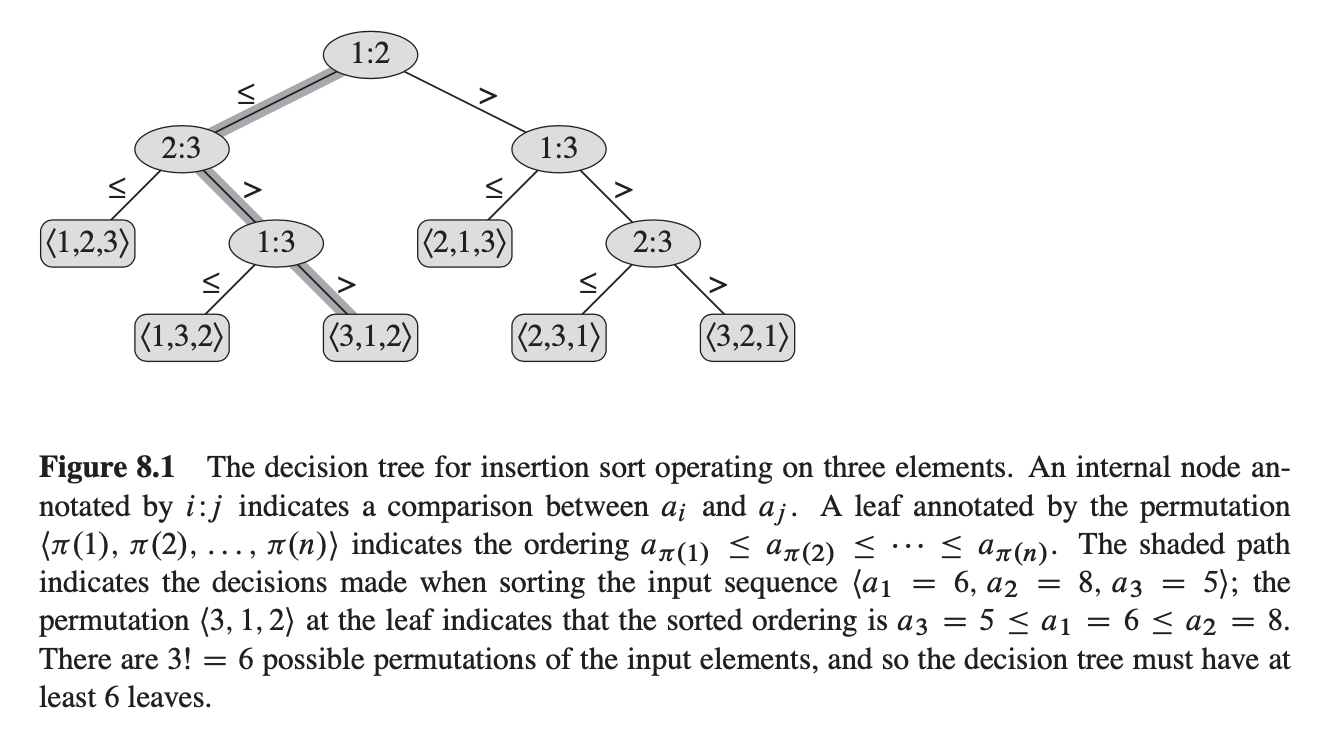
\includegraphics[scale=0.7]{images/decision_tree.png}

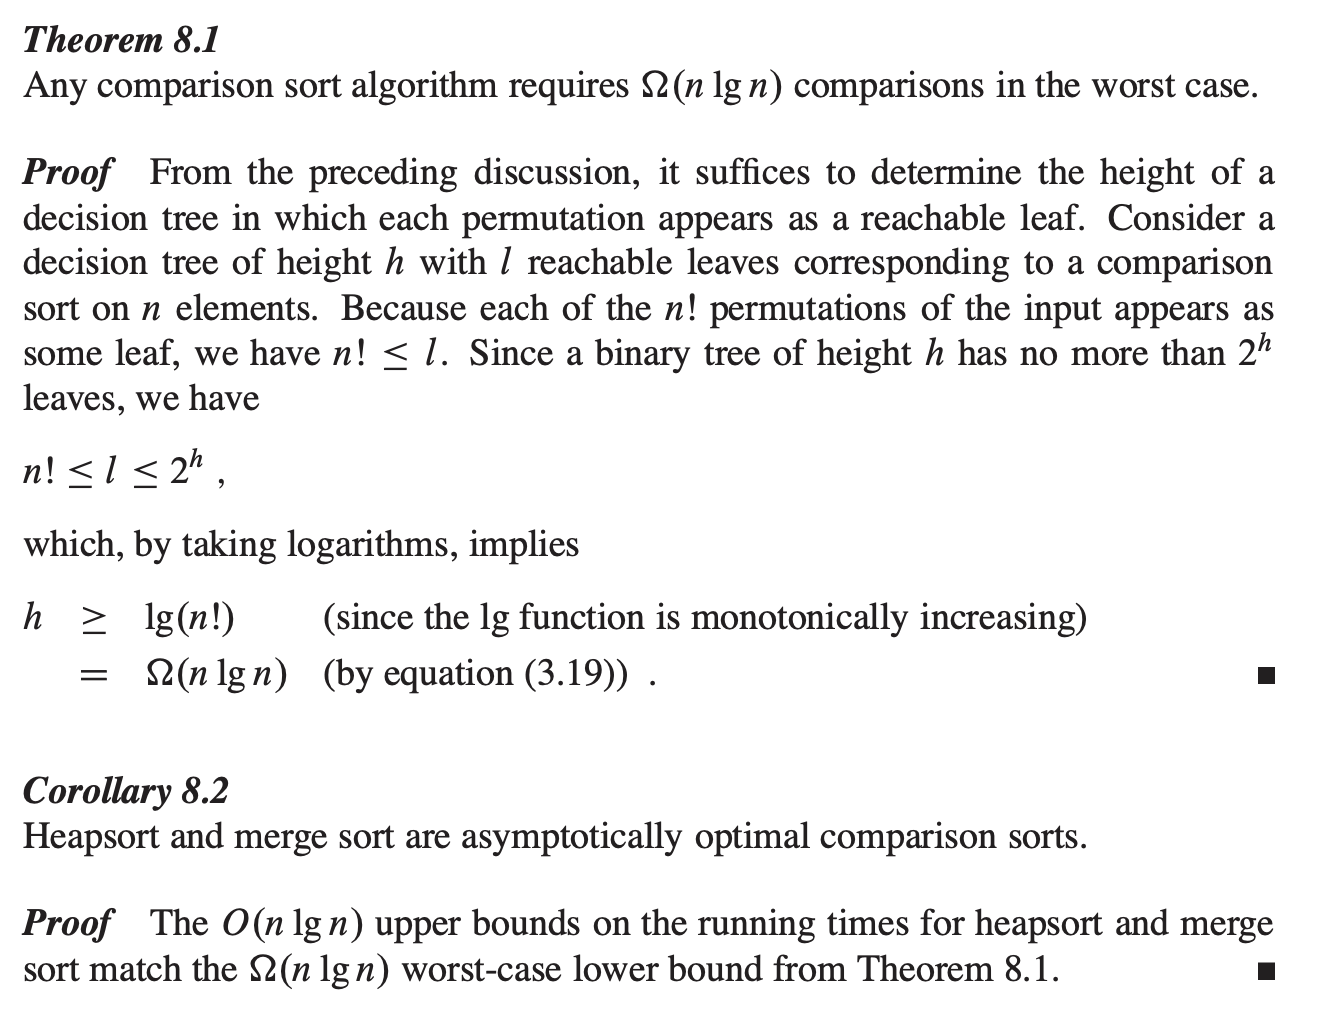
\includegraphics[scale=0.7]{images/theorem_8.1.png}
\newpage 

\section*{Matrix Chain Multiplication}
\subsection*{Step 1: Characterize Structure of an Optimal Solution}
Take \(i \leq j\) and let \(A_{i \dots j}\) denote the product \(A_i A_{i+1} \cdots A_j\).  If 
\(i = j\) then we already have an optimal solution for this case, because it requires no more 
computation.  If \(i<j\), then we can take some \(k\) where \(i \leq k < j\), and compute the 
multiplication \(A_{i \dots k}\) and \(A_{k+1 \dots j}\), then multiply them together.  The cost 
of this parenthesization is the cost to compute \(A_{i \dots k}\) plus the cost to compute 
\(A_{k+1 \dots j}\), plus the cost to multiply them together.

Suppose, to optimally parenthesize \(A_{i \dots j}\), we split the product between \(A_k\) and 
\(A_{k+1}\).  The multiplication \(A_i \dots A_k\) must have an optimal parenthesization, otherwise 
we could take a less costly parenthesization of \(A_i \dots A_k\), which would mean there'se a 
less costly way to parenthesize \(A_{i \dots j}\), but this is a contradiction, thus any subchain 
of \(A_{i \cdots j}\) must be an optimal parenthesization without loss of generality.

\subsection*{Step 2: Recursively define the value of an optimal solution}
Now we define the cost of an optimal solution recursively in terms of the cost of it's subproblems.
Let \(m[i,j]\) denote the minimum number of scalar multiplications to compute the matrix 
\(A_{i \dots j}\), so the lowest cost of the whole problem is \(m[1,n]\).  If \(i=j\) then no 
scalar multiplications, so \(m[i,j] = 0\).  If \(i < j\) then we can use the structure of our 
optimal solution.  Assuming the optimal split of our multiplication is between \(A_k\) and 
\(A_{k+1}\), then we get that \(m[i,j] = m[i,k] + m[k+1,j] + p_{i-1}p_kp_j\). \(p_{i-1}p_kp_j\) 
represents the number of scalar multiplications for \(A_{i \dots k}A_{k \dots j}\).  Since we 
don't actually know \(k\) we get the following recurrance definition\dots
\[m[i,j] = \begin{cases}
  0 & \text{if } i = j, \\
  \displaystyle\min_{i \leq k < j} \{m[i,k] + m[k+1,j] + p_{i-1}p_kp_j\}, & \text{if } i < j.
\end{cases}\]
We must also define \(s[i,j]\) to be the value of \(k\) at which the split at \(A_k,A_{k+1}\) 
yields the optimal parenthesization.  Without this, we won't actually be able to find our solution.

\subsection*{Step 3: Compute the value of an optimal solution}
Dynamic programming is meant for two specific cases.  The first is optimal substructure, and the 
second is overlapping subproblems, which this problem has a lot of.  Instead of recursion, we can 
use the tabular, bottom-up approach.  

Assuming matrix \(A_i\) has dimensions \(p_{i-1} \times p_i\), the input of our 
\proc{Matrix-Chain-Order} formula will be a sequence \(p = \langle p_0, \dots, p_n \rangle\).  
The algorithm will use auxiliary table \(m[i,j]\) for storing costs, and auxiliary table  \(s[i,j]\)
for actually constructing the optimal solution. 

To actually implement the bottom-up approach, we must determine entries of the table we refer to 
when computing \(m[i,j]\).  We know the cost of computing \(A_{i \dots j}\) is dependent on the 
cost of computing \(A_{i \dots k}\) and \(A_{k+1 \dots j}\) for some \(i \leq k < j\).  This means 
the cost of \(A_{i \dots j}\) depends only on the cost of matrix-chain-products of fewer matrices. 
So we must fill in table \(m\) in a manner that corresponds to increasing length of matrix chain 
multiplications.
\newpage
\begin{codebox}
  \Procname{\(\proc{Matrix-Chain-Order}(p)\)}
  \li n = \attrib{p}{length} - 1
  \li let \(m[1 \dots n, 1 \dots n]\) and \(s[1 \dots n, 1 \dots n]\) be new tables
  \li \For \(i \gets 1\) \To \(n\) \Do 
    \li \(m[i,i] \gets 0\) \End
  \li \For \(l \gets 2\) \To \(n\) \Comment \(l\) is the chain length
    \li \Do \For \(i \gets 1\) \To \(n-l+1\)
      \li \Do \(j \gets i+l-1\)
      \li \(m[i,j] \gets \infty\)
      \li \For \(k \gets i\) \To \(j-1\) \Do
        \li \(q \gets m[i,k] + m[k+1,j] + p_{i-1}p_kp_j\)
        \li \If \(q < m[i,j]\)
          \li \Then \(m[i,j] \gets q\)
          \li \(s[i,j] \gets k\) \End \End \End \End
  \li \Return \(m\) and \(s\)
\end{codebox}
This is bottom up, because we first assign 0 to all 1-length chains, then take a new chain length 
of 2, compute every possible multiplication and assign them to their corresponding locations in 
\(m\).  We keep repeating this loop, increasing the chain length until we find the solution for 
our entire procedure.

This is done in \(\Theta(n^3)\) time, with \(\Theta(n^2)\) space, which is much better than the 
exponential brute-force approach.

\subsection*{Step 4: Construct an optimal solution from computed information}
We made sure to also keep track of an extra auxiliary array \(s\) to store the actual locations 
of our splits for an optimal parenthesization.  \(s[i,j]\) records the value of \(k\) such that 
an optimal parenthesization of \(A_i A_{i+1} \cdots A_j\) splits the product between \(A_k\) and 
\(A_{k+1}\).  So to compute \(A_{1 \dots n}\) optimally, we must take 
\(A_{1 \dots k}A_{k+1 \dots n} = A_{1 \dots s[i,j]}A_{s[i,j]+1 \dots n}\).  Then to find the 
value where the two subproblems are split, we check \(s[1,k] = s[1,s[1,n]]\) and 
\(s[k+1,n] = s[s[1,n]+1,n]\). 

The following algorithm will print the optimal parenthesization of 
\(\langle A_i, A_{i+1}, \dots A_j \rangle\).  The initial call to \proc{Print-Optimal-Parens} 
should be \(i=1\) and \(j=n\).

\begin{codebox}
  \Procname{\(\proc{Print-Optimal-Parens}(s,i,j)\)}
  \li If \(i \isequal j\) \Then 
  \li print ``\(A\)''\(_i\) \End 
  \li \Else print ``('' \Then
    \li \(\proc{Print-Optimal-Parens}(s,i,s[i,j])\)
    \li \(\proc{Print-Optimal-Parens}(s,s[i,j]+1,j)\)
    \li print ``)'' \End
\end{codebox}

In order for us to use optimal substructure for a problem, our subproblems must always be 
independent.  Meaning that the solution to one subproblem must not affect another.  Shorts 
paths for vertices has independent subproblems, but not longest paths.  Dynamic programming 
solutions also need overlapping subproblems so it can solve it once, then store the answe in 
an auxiliary array where it can be looked up when needed, using constant-time lookup.
\newpage 

Using regular recursion to solve the matrix chain multiplication problem actually takes 
\(\Theta(2^n)\) time because subproblems are called multiple times, and subsequent calling 
of subproblems isn't linear like our above bottom-up approach.  Also when reconstructing the 
optimal solution, it's crucial to keep the \(s[i,j]\) table to keep track of the actuall values, 
without this table it becomes a bit slower to recall back with only the \(m[i,j]\) table.

Memoization takes the top-down approach of regular recursion, but also implements a table like 
in the more efficient bottom-up approach.  Each table entry initially contains a value to indicate 
that it hasn't been filled out yet.  When the subproblem is first encountered as the recursive 
algorithm unfolds, it's solution is computed, then stored in the table, then any subsequent lookup 
can just be found in the table from then on.

\begin{codebox}
  \Procname{\(\proc{Memoized-Matrix-Chain}(p)\)}
  \li \(n \gets \attrib{p}{length}-1\)
  \li let \(m[1 \dots n, 1 \dots n]\) be a new table
  \li \For \(i \gets 1\) \To \(n\) \Do
    \li \For \(j \gets 1\) \To \(n\) \Do
      \li \(m[i,j] \gets \infty\) \End \End
  \li \Return \(\proc{Lookup-Chain}(m,p,1,n)\)
\end{codebox}

\begin{codebox}
  \Procname{\(\proc{Lookup-Chain}(m,p,i,j)\)}
  \li \If \(m[i,j] < \infty\) \Then 
    \li \Return \(m[i,j]\) \End
  \li \If \(i \isequal j\) \Then 
    \li \(m[i,j] \gets 0\) \End
  \li \Else \For \(k \gets i\) \To \(j-1\) \Then \Do
      \li \(q \gets \proc{Lookup-Chain}(m,p,i,k)\)
      \zi \(\quad\quad + \proc{Lookup-Chain}(m,p,k+1,j)\)
      \zi \(\quad\quad + p_{i-1}p_kp_j\)
      \li \If \(q < m[i,j]\) \Then 
        \li \(m[i,j] \gets q\) \End \End \End 
  \li \Return \(m[i,j]\)
\end{codebox}

It first checks to see if the value is less than infinity, if so, then it just returns the value 
because this part of the table has already been computed.  Then it goes through and recursively 
calls \proc{Lookup-Chain} which will recurse all the way to the cases where \(i \isequal j\), and 
plop down a 0.  Then the recursion works it's way back, adding in new values to \(m\) as the call 
stack reduces.  

You can think of the bottom-up tabular approach as a sort of breadth-first-search, and the 
top-down memoization approach as a sort of depth-first search.
\newpage 

\section*{Longest Common Subsequence}
\subsection*{Step 1: Characterizing a longest common subsequence}
Given a sequence \(X = \langle x_1, x_2, \dots, x_m \rangle\) and sequence 
\(Y = \langle y_1, y_2, \dots, x_n \rangle\).  We will let 
\(Z = \langle z_1, z_2, \dots, z_k \rangle\) be any LCS of \(X\) and \(Y\).

\subsubsection*{Theorem (Optimal Substructure of an LCS)}
\begin{enumerate}
  \item If \(x_m = y_n\), then \(z_k = x_m = y_n\), and \(Z_{k-1}\) is an LCS of \(X_{m-1}\) and \(Y_{n-1}\).
  \item If \(x_m \not= y_n\), then \(z_k \not= x_m\) implies \(Z\) is an LCS of \(X_{m-1}\) and \(Y\).
  \item If \(x_m \not= y_n\), then \(z_k \not= y_n\) implies \(Z\) is an LCS of \(X\) and \(Y_{n-1}\).
\end{enumerate}
\subsubsection*{Proof}
For (1), if \(z_k \neq x_m\) then we could append \(x_m = y_n\) to \(Z\) to get a solution of length 
\(k+1\), this contradicts \(Z\) being the longest common subsequence.  Now we have that \(Z_{k-1}\) 
is a common subsequence of \(X_{m-1}\) and \(Y_{n-1}\).  Suppose that theres a subsequence 
\(W_{k-1}\) that's longer than \(Z_{k-1}\), then appending \(x_m = y_n\) gives us a longer subsequence 
which is again a contradiction.

Without loss of generality, for (2) and (3), if \(z_k \neq x_m\) then \(Z\) is a common subsequence 
of \(X_{m-1}\) and \(Y\).  Suppose there's a subsequence \(W\) of \(X_{m-1}\) and \(Y\) with length 
greater than \(k\), then \(W\) is also a subsequence of \(X\) but this is a contradiction because 
the LCS of \(X\) and \(Y\) is of length \(k\).  Therefore, since an LCS of two sequences contains 
an LCS of the prefixes of the two sequences, this problem has optimal substructure.

\subsection*{Step 2: A recursive solution}
When \(x_m = y_n\), we must find the LCS of \(X_{m-1}\) and \(Y_{n-1}\), and appending  \(x_m = y_n\) 
gives us the LCS for \(X\) and \(Y\).  And when \(x_m \neq y_n\), there are possibilities we must 
cover.  We find the LCS of \(X_{m-1}\) and \(Y\) and we find the LCS of \(X\) and \(Y_{n-1}\).  
Whichever one is longer is the one we use for the LCS of \(X\) and \(Y\).  

We also have overlapping subproblems, because if we must find LCS of \(X_{m-1}\) and \(Y\) and LCS 
of \(X\) and \(Y_{n-1}\), then they may share an LCS subproblem of \(X_{m-1}\) and \(Y_{n-1}\). 
Lots of other subproblems also share subproblems.  Our recursive solution to LCS involves establishing 
a recurrance for the value of an optimal solution.  Let \(c[i,j]\) be the lenghth of the LCS of 
\(X_i\) and \(Y_j\), this gives us the following recurrence\dots 

\[c[i,j] = \begin{cases}
  0 & \text{if } i=0 \text{or} j=0, \\ 
  c[i-1,j-1] + 1 & \text{if } i,j > 0 \text{and} x_i = y_j, \\ 
  \max \big(c[i-1,j], c[i,j-1]\big) & \text{if } i,j > 0 \text{and} x_i \neq y_j.
\end{cases}\]

LCS is actually a problem that rules out subproblems depending on the conditions of the problem.  
For example, if \(x_i = y_j\) then we only check the subproblem of finding the LCS of  \(X_{i-1}\) 
and \(Y_{j-1}\).  But if \(x_i \neq y_j\), then we actually have two subproblems.
\newpage

\subsection*{Step 3: Computing the length of an LCS}
The LCS problem has very few distinct subproblems, so we can use dynamic programming to compute 
the solutoin bottom up. \proc{LCS-Length} takes two inputs, \(X = \langle x_1,x_2,\dots,x_m \rangle\), 
and \(Y = \langle y_1,y_2,\dots,y_n \rangle\).  Stores the LCS values for \(X_i\) and \(Y_j\) in 
\(c[i,j]\).  It will also use \(b[1 \dots m, 1 \dots n]\) to help construct our optimal solution.

\(b[i,j]\) will point to the entry containing the optimal subproblem solution, so if 

\begin{codebox}
  \Procname{\(\proc{LCS-Length}(X,Y)\)}
  \li m = \attrib{X}{length}
  \li n = \attrib{Y}{length}
  \li let \(b[1 \dots m, 1 \dots n]\) and \(c[0 \dots m, 0 \dots n]\) be new tables
  \li \For \(i \gets 0\) \To \(m\) \Do
    \li \(c[i,0] \gets 0\) \End
  \li \For \(j \gets 0\) \To \(n\) \Do
    \li \(c[0,j] \gets 0\) \End
  \li \For \(i \gets 1\) \To \(m\) \Do
    \li \For \(j \gets 1\) \To \(n\) \Do
      \li \If \(x_i \isequal y_j\) \Then 
        \li \(c[i,j] \gets c[i-1,j-1] + 1\)
        \li \(b[i,j] \gets ``\nwarrow"\)
      \li \ElseIf \(c[i-1,j] > c[i,j-1]\) \Then 
        \li \(c[i,j] \gets c[i-1,j]\)
        \li \(b[i,j] \gets ``\uparrow"\)
      \li \Else \(c[i,j] \gets c[i,j-1]\)
        \li \(b[i,j] \gets ``\leftarrow"\)
        \End \End \End 
  \li \Return \(c\) and \(b\)
\end{codebox}

\subsection*{Step 4: Constructing an LCS}
Now that we have our auxiliary table \(b\) all we need to do is start at \(b[m,n]\) and work 
our way back, printing a letter every time we encounter a ``\(\nwarrow\)''.  But we don't want to 
print our LCS in reverse order, so we'll use tail recursion, actually adding the letter after 
the recursive call.

\begin{codebox}
  \Procname{\(\proc{Print-LCS}(b,X,i,j)\)}
  \li \If \(i \isequal 0\) or \(j \isequal 0\) \Then 
  \li \Return \End 
  \li \If \(b[i,j] \isequal ``\nwarrow"\) \Then 
    \li \(\proc{Print-LCS}(b,X,i-1,j-1)\)
    \li print \(x_i\)
  \li \ElseIf \(b[i,j] \isequal ``\uparrow"\) \Then
    \li \(\proc{Print-LCS}(b,X,i-1,j)\)
  \li \Else \(\proc{Print-LCS}(b,X,i,j-1)\) \End
\end{codebox}

We only need \(X\) for this because we're finding a substring, so either one would work.  Also 
to get the whole LCS with the above function, we would call 
\(\proc{Print-LCS}(b,X,\attrib{X}{length},\attrib{Y}{length})\).
\newpage 

\section*{Activity Selection Problem}
Given a set of activities \(S = \{a_1, a_2, \dots, a_n\}\) with \(a_i\)'s corresponding start 
and finish times \(s_i\) and \(f_i\), we want to find the largest numbers of non-overlapping 
activities. Take \([s_i,f_i)\) and \([s_j,f_j)\), they're compatible if \(s_j \geq f_i\) or if 
\(s_i \geq f_j\).

\subsection*{Optimal substructure of activity-selection}
Let \(S_{ij}\) denote the set of activities that start during or after \(f_i\) and finish before 
\(s_j\).  Also let \(A_{ij}\) be the maximum non-overlapping activity set for \(S_{ij}\).  If 
\(A_{ij}\) has activity \(a_k\), then we can split into two subproblems, giving us 
\(A_{ij} = A_{ik} \cup \{a_k\} \cup A_{kj}\), and the maximum sized set \(A_{ij}\) has 
\(|A_{ik}| + |A_{kj}| + 1\) activities.

If we find an \(A'_{ik}\) where \(|A'_{ik}| > |A_{ik}|\) then we could could substitute it in 
to find \((A'_{ij}\) where \(|A'_{ij}| > |A_{ij}|\) which is a contradiction, because we assume 
\(A_{ij}\) is a maximal set of activities.  This means that dynamic programming may be a good idea.

Letting \(c[i,j]\) represent the size of the optimal solution for \(S_{ij}\) we get that\dots 

\[c[i,j] = \begin{cases}
  0 & \text{if } S_{ij} = \emptyset, \\ 
  \displaystyle\max_{a_k \in S_{ij}} \big(c[i,k] + c[k,j] + 1\big) & \text{if } S_{ij} \neq \emptyset.
\end{cases}\]

\subsection*{Making the greedy choice}
We must choose the activity that leaves resources available for as many other activities as possible. 
Let's choose our greedy choice to be the activity with the earliest finish time.  Since the 
activities are sorted in monotonically increasing order by finish time, our greedy choice is \(a_1\). 

Making the greedy choice leaves one subproblem, finding activities starting after \(a_1\) finishes. 
Let \(S_k = \{a_i \in S : s_i \geq f_k\}\) be the set of activities starting after \(a_k\) finishes. 
Greedy choice \(a_1\) leaves subproblem \(S_1\).  Now we must see if this greedy choice does 
actually yield an optimal solution.

\subsubsection*{Theorem}
Consider non-empty subproblem \(S_k\), and let \(a_m\) be the activity with the earliest finish 
time in \(S_k\).  Then \(a_m\) is in a maximum mutually-exclusive subset of \(S_k\).

\subsubsection*{Proof}
Let \(A_k\) be a maximum size subset of \(S_k\) and let \(a_j\) be the activity with the earliest 
finish time in \(A_k\).  If \(a_k = a_m\) then the optimal solution contains our greedy choice, 
and we are done.  Otherwise, we can let \(A'_k = A_k - \{a_j\} \cup \{a_m\}\).  The activities 
in \(A'_k\) are disjoint because \(A_k\) is disjoint, \(a_j\) is the first activity in \(A_k\) 
to finish, and \(f_m \leq f_j\).  Therefore, since \(|A'_k| = |A_k|\), we have a new solution to 
the problem which now contains our greedy choice.

\n 
Finding a greedy algorithm approach can work using the top-down method, because we can simply choose 
an activity to put into our optimal solution, then recursively find the next activity.  Greedy 
algorithms usually work top-down, where you make a choice, then solve the subproblem, as opposed 
to the bottom-up approach.
\newpage 

\subsection*{Recursive greedy algorithm}
we can now write a straightforward recursive algorithm to find the maximum disjoint set of 
activities. \proc{Recursive-Activity-Selector} takes arrays \(s\) and \(f\) for start and finish 
times, index \(k\) representing the \(S_k\) subproblem, and size \(n\) of the original problem.  
We assum the \(n\) activities are sorted by finish time.  To start the recursive call, we create 
activity \(a_0\) with finish time \(f_0 = 0\) so \(S_0\) contains all the activities.  So our 
call is \(\proc{Recursive-Activity-Selector}(s,f,0,n)\).

\begin{codebox}
  \Procname{\(\proc{Recursive-Activity-Selector}(s,f,k,n)\)}
  \li \(m \gets k+1\)
  \li \While \(m \leq n\) and \(s[m] < f[k]\) \Comment find first activity in \(S_k\) to finish
    \li \Do \(m \gets m+1\) \End 
  \li \If \(m \leq n\) \Then 
    \li \Return \(\{a_m\} \cup \proc{Recursive-Activity-Selector}(s,f,m,n)\) 
  \li \Else \Return \(\emptyset\) \End
\end{codebox}
This algorithm has a running time of \(\Theta(n)\) because every element of \(S\) is checked 
once.  If the while look stops at some element \(k\), then the next recursive call picks up 
right where the previous one left off, thus iterating through every activity once.

\subsection*{Iterative greedy algorithm}
Since the recursive call in the above greedy algorithm is called at the end of the function, we 
can actually use an iterative approach for this problem as well.  This type of recursion is 
called tail recursion, and is actually quite easy to turn into an iterative algorithm.  Some 
compilers will actually automatically turn a tail-recursive algorithm into an iterative one. 
\proc{Greedy-Activity-Selector} assumes activities are sorted and creates a set \(A\) 
containing the activities, returning it at the end.

\begin{codebox}
  \Procname{\(\proc{Greedy-Activity-Selector}(s,f)\)}
  \li \(n \gets \attrib{s}{length}\)
  \li \(A \gets \{a_1\}\)
  \li \(k \gets 1\)
  \li \For \(m \gets 2\) \To \(n\) \Do
    \li \If \(s[m] \geq f[k]\) \Then 
      \li \(A \gets A \cup \{a_m\}\)
      \li \(k \gets m\) \End \End
  \li \Return \(A\)
\end{codebox}

This algorithm essentially does the same thing as calling \(\proc{Recursive-Activity-Selector}(s,f,0,n)\). 
And You can now, more obviousely, see that the running time is \(\Theta(n)\).
\newpage 

\section*{Elements of a Greedy Strategy}
The heuristic greedy approach doesn't always work, but there are specific cases that it does. 
If you want to fashion a solution to a problem with a greedy choice in mind, then you can follow 
these steps\dots 

\begin{enumerate}
\item Cast the optimization problem as one in which we make a choice and are left with one subproblem 
  to solve.
\item Prove that there is always an optimal solution to the problem that contains the greedy choice, 
  thus making the greedy choice safe.
\item Demonstrate optimal substructure by showing that, having made the greedy choice, what remains 
  is a subproblem with the property that combining the optimal solution to the subproblem with our 
  greedy choice yields an optimal solution.  Inductively, this shows that making the greedy choice 
  at every inductive step also yields an optimal solution.
\end{enumerate}

\subsection*{Greedy-choice propety}
In dynamic programming, we usually make a choice at every step, but that choice usually depends on 
solutions to subproblems.  This is why dynamic programming usually works bottom-up.  Unless we 
want to use memoization, which technically works top-down, but still must first answer subproblems. 
With greedy algorithms, we just make a choice that seems right, then solve the remaining 
subproblem.  Greedy algorithm choices may depend on previous choices, but never depend on 
solutions to subproblems.  Therefore, greedy algorithms actually do work top-down.  Proving 
that greedy algorithms work is usually done by taking a global optimal solution, replacing a choice 
with the greedy choice, and showing that it's still an optimal solution.

\subsection*{Optimal substructure}
A problem exhibits optimal substructure if an optimal solution to a problem contains within it 
optimal solutions to subproblems.  For greedy algorithms, all we really need to prove optimality is 
to prove that an optimal solution to the subproblem, combined with the greedy choice yields an 
optimal solution to the original problem.

\subsection*{Greedy vs dynamic programming}
Not all problems can be solved using a greedy algorithm.  For example, take the knapsack problem. 
For the 0-1 knapsack problem and the fractional knapsack problem, they both contain optimal 
substructure, but only one can be solved using a greedy algorithm.

For the fractional knapsack problem, if we take our greedy choice to be the item with the most 
valuable density, then taking as much of that before running out (or running out of space in 
the knapsack), then this solution is optimal.  

For the 0-1 knapsack problem though, take items \(o_1, o_2, o_3\) with \(w_1=10, w_2=20, w_3=30\) 
and \(c_1=60, c_2=100, c_3=120\).  Also assume knapsack holds 50 lbs.  Greedy strategy would be 
to take objects with highest money density, which is \(o_1\) and \(o_2\).  If we also put \(o_3\) 
in the sack, we have too much weight, so we can only carry the first two.  This gives us a price 
of \$160.  But the actual optimal solution is to take \(o_2\) and \(o_3\), this hits our 
knapsack weight perfectly, and gives us a price of \$220.  So not all problems can be solved with 
greedy algorithms.
\newpage

\section*{Huffman Codes}
Huffman's greedy algorithm takes in a table of character counts and produces a variable length 
bit sequence for each character. It does this with \textbf{\textit{prefix codes}}: no codeword is 
a prefix of another.  Prefix codes help simplify decoding.  We just identify a codeword, convert 
it to it's corresponding character, then move on to the rest of the prefix code.

To optimally represent the prefix code, we must use a full binary tree, where every internal node 
has two children.  Given a tree \(T\) corresponding to a prefix code, we can compute the number of 
bits needed to encode a file.  For any leter \(c\) in alphabet \(C\), we can let \(d_T(c)\) 
denote the depth of \(c\)'s leaf in \(T\).  So to find the number of bit's needed to encode a 
file, we use this equation\dots 
\[\sum_{c \in C} \attrib{c}{freq} \cdot d_T(c)\]

\subsection*{Constructing a Huffman code}
Assuming \(C\) is a set of \(n\) characters, the algorithm \(\proc{Huffman}(C)\) builds the tree 
\(T\) corresponding to the optimal code bottom-up.  Starts with \(|C|\) leaves, and merges them 
\(|C|-1\) times to create the final tree.  We must use a min-priority-queue \(Q\) sorted by 
\attrib{c}{freq}.  We take the two least frequent characters and merge them, we work upwards 
until everything is merged, and more frequent characters have less depth.

\begin{codebox}
  \Procname{\(\proc{Huffman}(C)\)}
  \li \(n \gets |C|\)
  \li \(Q \gets C\)
  \li \For \(i \gets 1\) \To \(n-1\) \Do
    \li allocate new node \(z\)
    \li \(\attrib{z}{left} \gets x \gets \proc{Extract-Min}(Q)\)
    \li \(\attrib{z}{right} \gets y \gets \proc{Extract-Min}(Q)\)
    \li \(\attrib{z}{freq} \gets \attrib{y}{freq} + \attrib{y}{freq}\)
    \li \(\proc{Insert}(Q,z)\) \End 
  \li \Return \(\proc{Extract-Min}(Q)\) \Comment return root of tree
\end{codebox}

Initializing the min-heap \(Q\) is \(O(n)\) with the \proc{Build-Min-Heap} procedure.  Then we 
iterate through the for-loop which is \(O(n)\).  Inside each for loop iteration, we call 
\proc{Extract-Min} twice and \proc{Insert} once, all of these are \(O(\lg n)\) operations, so this 
makes the whole \proc{Huffman} algorithm run in \(O(n \lg n)\) time.

\subsection*{Correctness of Huffman's algorithm}
To prove that this Huffman's algorithm is correct we must show that the problem of an optimal 
prefix code exhibits a greedy-choice and optimal substructure property.

\begin{greedy}
  Let \(x\) and \(y\) be two characters in \(C\) having lowest frequencies. Then there exists an 
  optimal prefix code where \(x\) and \(y\) have the same length and only differ in the last bit. 
  Proof on the next page.
\end{greedy}
\newpage 
\begin{proof}
  Let \(a\) and \(b\) be two sibling leaves of max depth on tree \(T\).  WLOG, we assum 
  \(\attrib{a}{freq} \leq \attrib{b}{freq}\) and \(\attrib{x}{freq} \leq \attrib{y}{freq}\).
  Since \(x\) and \(y\) are the lowest frequency leaves, we know 
  \(\attrib{x}{freq} \leq \attrib{a}{freq}\) and \(\attrib{y}{freq} \leq \attrib{b}{freq}\).
  If they're equal, then lour lemma holds, as our greedy choice already does yield an optimal 
  solution.

  So let's assume \(x \neq b\).  Now we can take tree \(T\) replacing \(x\) with \(a\) making 
  a new tree \(T'\).  Then replacing \(y\) with \(b\) giving us \(T''\).  We can take size of 
  a file from \(T\) and subtract the size of a file from \(T'\) to show \(T'\) cannot be greater. 

  \begin{align*}
    && B(T)-B(T') &= \sum_{c \in C} \attrib{c}{freq} \cdot d_T(c) - 
    \sum_{c \in C} \attrib{c}{freq} \cdot d_{T'}(c) && \\
    && &= \attrib{x}{freq} \cdot d_T(x) + \attrib{a}{freq} \cdot d_T(a)
         -\attrib{x}{freq} \cdot d_{T'}(x) - \attrib{a}{freq} \cdot d_{T'}(a) && \\ 
    && &= \attrib{x}{freq} \cdot d_T(x) + \attrib{a}{freq} \cdot d_T(a)
         -\attrib{x}{freq} \cdot d_T(a) - \attrib{a}{freq} \cdot d_T(x) && \\ 
    && &= (\attrib{a}{freq} - \attrib{x}{freq}) \cdot (d_T(a) - d_T(x)) && \\
    && &\geq 0
  \end{align*}

  So since \(B(T') \leq B(T)\), and WLOG, \(B(T'') \leq B(T')\), we have \(B(T'') \leq B(T)\), 
  And since \(T\) is an optimal tree, \(B(T'') \geq B(T)\), so it must also be the case that 
  \(T''\) is also an optimal tree.
\end{proof}

\begin{substructure}
  Let \(C'\) be the alphabet with characters \(x\) and \(y\) removed and new character \(z\)
  added where \(\attrib{z}{freq} \gets \attrib{y}{freq} + \attrib{y}{freq}\). Let \(T'\) be any 
  tree representing optimal prefix code for \(C'\). Then the tree \(T\) obtained from \(T'\) by 
  replacing the leaf node for \(z\) with an internal node containing \(x\) and \(y\) as children, 
  represents an optimal prefix code for \(C\).
\end{substructure}

\begin{proof}
  We first must express the cost \(B(T)\) in terms of \(B(T')\).  First note that for any 
  \(c \in C - \{x,y\}\), \(d_T(c) = d_{T'}(c)\). Also \(d_T(x) = d_T(y) = d_{T'}(z)+1\). So we 
  get \(B(T) = B(T') + \attrib{x}{freq} + \attrib{y}{freq}\). 

  Now, suppose to the contrary, that \(T\) is not an optimal prefix code for \(C\).  Then there 
  exists tree \(T''\) such that \(B(T'') < B(T)\).  \(x\) and \(y\) are siblings in this tree 
  because of the previous lemma, so if we take \(T'''\) wheren \(x\) and \(y\) are replaced by 
  node \(z\) then we get the following relation\dots 

  \begin{align*}
    && B(T''') &= B(T'') - \attrib{y}{freq} - \attrib{y}{freq} && \\
    && &\leq B(T) - \attrib{y}{freq} - \attrib{y}{freq} && \\
    && &= B(T')
  \end{align*}
  But since we assumed that \(T'\) represents an optimal prefix code, we have a contradiction, so 
  it must be the case that \(T\) represents an optimal prefix code of \(C\).
\end{proof}

\begin{huffman}
  The \proc{Huffman} algorithm produces optimal prefix code.
\end{huffman}
\begin{proof}
  look at previous lemmas.
\end{proof}
\newpage 
\section*{Disjoint set forests}
\begin{codebox}
  \Procname{\(\proc{Make-Set}(x)\)}
  \li \(\attrib{a}{p} \gets x\)
  \li \(\attrib{x}{rank} \gets 0\)
\end{codebox}

\begin{codebox}
  \Procname{\(\proc{Union}(x,y)\)}
  \li \(\proc{Link}(\proc{Find-Set}(x), \proc{Find-Set}(y))\)
\end{codebox}

We use union by rank to ensure our sets don't get unnecessarily long.  We take the longer of the 
two sets and use their root as the root of the new set.

\begin{codebox}
  \Procname{\(\proc{Link}(x,y)\)}
  \li \If \(\attrib{x}{rank} > \attrib{y}{rank}\) \Then 
    \li \(\attrib{y}{p} \gets x\)
  \li\Else \(\attrib{x}{p} \gets y\)
    \li \If \(\attrib{x}{rank} \isequal \attrib{y}{rank}\) \Then 
      \li \(\attrib{y}{rank} \gets \attrib{y}{rank} + 1\) \End \End
\end{codebox}

We can use path compression for the \proc{Find-Set} operation, so every time we traverse down 
a set, we update the parents of each node to be the root of the set.  This makes subsequent calls 
to \proc{Find-Set} faster, thus also making \proc{Union} faster.

\begin{codebox}
  \Procname{\(\proc{Find-Set}(x)\)}
  \li \If \(\attrib{x}{p} \neq x\) \Then 
    \li \(\attrib{x}{p} \gets \proc{Find-Set}(\attrib{x}{p})\) \End
  \li \Return \attrib{x}{p}
\end{codebox}

Both the union by rank heuristic and the path compression heuristic improve our data structures 
slightly.  When implementing both, we get a running time of \(O(m\alpha(n))\), where \(\alpha\) 
is a very slowly growing function.  This basically means running time is linear.

\section*{Representation of graphs}
You can represent graphs as a list or a matrix.  For sparce graphs (less edges), a list is a 
better representation, as it takes up much less space.  But all-pairs shortest path algorithm 
uses matrices because edges are more dense.

\textbf{\textit{Adjacency lists}} are represented as an array of \(|V|\) lists (one for each 
vertex), and each adjacency list \(Adj[u]\) contains nodes \(v\) st edge \((u,v) \in E\).  if 
\(G\) is directed, then sum of adjacency list lengths are \(|E|\), and \(2|E|\) for undirected 
graphs.  Space complexity is \(\Theta(|V|+|E|)\).  For storing weights, we can add a weight 
attribute \(w(u,v)\) with vertex \(v\) in \(u\)'s adjacency-list.

\textbf{\textit{Adjacency matrices}} on the other hand have \(\Theta(|V^2|)\) space complexity 
but they do have constant-time lookup for edges, where the list representation requires searching 
through the \(Adj[u]\) list.  Then for each element of the matrix, \(a_{ij}\) recieves a 1 if 
there exists an edge from \(i\) to \(j\) and a 0 otherwise.  This makes adding weight easy because 
we can instead just add \(w(i,j)\) to the entry.
\newpage

\section*{Minimum Spanning Trees}
\begin{codebox}
  \Procname{\(\proc{Generic-MST}(G,w)\)}
  \li \(A \gets \emptyset\)
  \li \While \(A\) does not form a minimum spanning tree \Do
    \li find an edge \((u,v)\) that's safe for \(A\) 
    \li \(A \gets A \cup \{(u,v)\}\) \End
  \li \Return \(A\)
\end{codebox}

\textbf{\textit{cut}}: \((S,V-S)\) is a cut of \(G\) if it partitions \(G\) into two sets of 
vertices.

\textbf{\textit{cross}}: an edge \((u,v)\) crosses the cut if \(u \in S\) and \(v \in V-S\) or 
vice versa.

\textbf{\textit{respect}}: a cut respects a set \(A\) of edges, if no edge in \(A\) crosses 
said cut.

\textbf{\textit{light edge}}: an edge is a light edge if it's the minimum weight of any edge that 
crosses the cut.

\textbf{\textit{safe edge}}: an ege that can be added to \(A\) to keep a as a subset of some MST.

\begin{safe}
  If \(A \subseteq E\) in some minimum spanning tree for \(G\).  Then take cut \((S, V-S)\) of \(G\) 
  that respects \(A\), if we append light edge \((u,v)\) crossing our cut to \(A\) then \(A\) is 
  still a subset of our MST \(G\), hence \((u,v)\) is safe for \(A\).
\end{safe}

\begin{proof}
  let \(T\) be an MST that includes \(A\) and doesn't include edge \((u,v)\). We create new MST 
  \(T'\) with \(A \cup \{(u,v)\}\), thus showing \((u,v)\) is safe for \(A\).  Since \(T\) is an 
  MST, if we add \((u,v)\) to \(T\), it would create a cycle with another edge \((x,y)\) crossing 
  cut \((S,V-s)\). 

  Since the cut respects \(A\), \((x,y)\) cannot be in \(A\).  If we remove \((x,y)\) from \(T\), 
  and add in \((u,v)\) we still have a tree because they cross the same cut.  So take 
  \(T' = (T-\{(x,y)\})\cup(u,v)\), now we show \(T'\) is a minimum spanning tree. 
  \(w(T') = w(T) - w(x,y) + w(u,v) \leq w(T)\).  Therefore \(T'\) must also be an MST, thus \((u,v)\) 
  is safe for \(A\).
\end{proof}

Now we go over two algorithms for making minimum spanning trees.  The first is Kruskal's algorithm, 
where the safe edge added is always the least-weight edge in the graph that connects two distinct 
components.  This basically creates tons of mini MST's before finally connecting everything into 
one big MST.

Prim's algorithm is the other. In this case our set \(A\) forms a single tree, and the safe edge 
added to \(A\) is always a least-weight edge connecting the existing tree to a vertex not in the 
tree.

\begin{codebox}
  \Procname{\(\proc{MST-Kruskal}(G,w)\)}
  \li \(A \gets \emptyset\)
  \li \For each vertex \(v \in \attrib{G}{V}\) \Do
    \li \(\proc{Make-Set}(v)\) \End
  \li sort edges of \attrib{G}{V} in increasing order by weight \(w\)
  \li \For each edge \((u,v)\in \attrib{G}{E}\) \Do
    \li \If \(\proc{Find-Set}(u) \neq \proc{Find-Set}(v)\) \Then
      \li \(A \gets A \cup \{(u,v)\}\)
      \li \(\proc{Union}(u,v)\) \End \End 
  \li \Return \(A\)
\end{codebox}

Assuming we're using the disjoint set forest data structure with our heuristics, we get the following 
complextiy.  Sorting the edges is done in \(O(E \lg E)\) time. The loop does \(O(E)\) 
\proc{Find-Set} and \proc{Union} operations. Along with the \(|V|\) \proc{Make-Set} calls, we get 
a running time of \(O(V+E)\alpha(V)\). Since \(|E| \geq |V|-1\), we get \(E\alpha(V)\), and since 
\(\alpha(V) = O(\lg V)\), we get that the overall running time is \(O(E \lg V)\).
\newpage 

For Prim's algorithm, we'll need a fast way to select a new edge for the tree, so we will need two 
new variables. We also keep a min-priority-queue queue for all the vertices that aren't in the tree 
yet. The queue is sorted by the vertices \id{key} attribute, which represents the weight of the 
minimum weight edge connecting our vertex to the tree. If there is no edge currently connecting an 
edge \(v\) to the tree, then we set \(\attrib{v}{key} = \infty\), and \(\attrib{v}{\pi} = \) NIL.
\(\pi\) represents the penultimate node with the property that \((v,v.\pi) = v.key\).  Finally 
when the algorithm terminates, we have an empty queue, because every vertex is in our tree.
\begin{codebox}
  \Procname{\(\proc{MST-Prim}(G,w,r)\)}
  \li \For each \(u \in \attrib{G}{V}\) \Do 
    \li \(\attrib{u}{key} \gets \infty\)
    \li \(\attrib{u}{\pi} \gets \) NIL \End 
  \li \(\attrib{r}{key} \gets 0\)
  \li \(Q \gets \attrib{G}{V}\)
  \li \While \(Q \neq \emptyset\) \Do 
    \li \(u \gets \proc{Extract-Min}(Q)\)
    \li \For each \(v \in \attrib{G}{Adj[u]}\) \Do 
      \li \If \(v \in Q\) and \(w(u,v) < \attrib{v}{key}\) \Then 
        \li \(\attrib{v}{\pi} \gets u\)
        \li \(\attrib{v}{key} \gets w(u,v)\) \End \End \End
\end{codebox}

For the running time, assuming we're using a min-heap for \(Q\), we must use the 
\proc{Build-Min-Heap} operation which is \(O(V)\) time.  The while loop executes \(|V|\) times, 
and \proc{Extract-Min} takes \(O(\lg V)\) time, so we get \(O(V \lg V)\) for that. The for loop 
is executed exactly \(|E|\) times, and since we must call \proc{Decrease-Key} every time the 
\id{key} value is adjusted, that's another \(O(\lg V)\) time.  So we get the the overall running 
time is \(O(V \lg V + E \lg V)\) = \(O(E \lg V)\), this is the same as for Kruskal's algorithm.

\section*{Single Source Shortest Path}
\begin{codebox}
  \Procname{\(\proc{Initialize-Single-Source}(G,s)\)}
  \li \For each vertex \(v \in \attrib{G}{V}\) \Do 
    \li \(\attrib{v}{d} \gets \infty\)
    \li \(\attrib{v}{\pi} \gets \) NIL \End
  \li \(\attrib{s}{d} \gets 0\)
\end{codebox}

\begin{codebox}
  \Procname{\(\proc{Relax}(u,v,w)\)}
  \li \If \(\attrib{v}{d} > \attrib{u}{d} + w(u,v)\) \Then
    \li \(\attrib{v}{d} \gets \attrib{u}{d} + w(u,v)\)
    \li \(\attrib{v}{\pi} \gets u\) \End
\end{codebox}
We will implement Dijkstra's algorithm on the next page.
\newpage 

\begin{codebox}
  \Procname{\(\proc{Dijkstra}(G,w,s)\)}
  \li \(\proc{Initialize-Single-Source}(G,s)\)
  \li \(S \gets \emptyset\)
  \li \(Q \gets \attrib{G}{V}\)
  \li \While \(Q \neq \emptyset\) \Do
    \li \(u \gets \proc{Extract-Min}(Q)\)
    \li \(S \gets S \cup \{u\}\)
    \li \For each \(v \in \attrib{G}{Adj[u]}\) \Do 
      \li \(\proc{Relax}(u,v,w)\) \End \End
\end{codebox}

This is a greedy strategy because the algorithm chooses the ligthest weight vertex in \(V-S\).

Now we can attempt to calculate the running time.  The for loop is called \(|E|\) times as it 
covers every edge for every vertex. So \proc{Decrease-Key} is called at most \(|E|\) times.
The while loop iterates \(|V|\) times, and \proc{Extract-Min} is \(O{\lg V}\).  Also building 
our heap is \(O(V)\), and each \proc{Decrease-Key} takes \(O(\lg V)\).  So we get a running time 
of \(O(V \lg V) + O(E \lg V) = O(E \lg V)\).

We can use a couple different data structures to achieve slightly better running times but this 
is essentially it.

\section*{All Pairs Shortest Path}
This algorithm takes the shortest \(1 \dots k\) length path, and computes the next shortest path 
up to \(k+1\) length

\begin{codebox}
  \Procname{\(\proc{Extend-Shortest-Paths}(L,W)\)}
  \li \(n \gets \attrib{L}{rows}\)
  \li let \(L' = (l'_{ij})\) be a new \(n \times n\) matrix
  \li \For \(i \gets 1\) \To \(n\) \Do
  \li \For \(j \gets 1\) \To \(n\) \Do
  \li \((l'_{ij}) \gets \infty\)
  \li \For \(k \gets 1\) \To \(n\) \Do
  \li \((l'_{ij}) \gets \min \{l'_{ij}, l_{ik} + w_{kj}\}\)
  \End \End \End 
  \li \Return \(L'\)
\end{codebox}
\[c_{ij} = \sum_{k=1}^n a_{ik} \cdot b_{kj} \quad\Rightarrow\quad
  l^{(m-1)}_{ij} = \displaystyle\min_{1 \leq k \leq n} l^{(m)}_{ik} + w_{kj}\]
  \[a \rightarrow l^{(m-1)} \quad\quad b \rightarrow w \quad\quad c \rightarrow  l^{(m)} 
  \quad\quad + \rightarrow \min \quad\quad \cdot \rightarrow +\]

We can start with the \(W\) matrix and call \proc{Extend-Shortest-Paths} \(n-1\) times to give 
us our all-pairs shortest paths matrix, and this can be done in \(O(V^4)\) time.  We can actually 
improve this by instead doing matrix multiplication on two \(W\) matrices, then multiple them 
together, and keep doing this until we reach a matrix power greater than or equal to \(n-1\). 
This makes the algorithm \(O(V^3 \lg V)\) and I'll show it on the next page.
\newpage

\begin{codebox}
  \Procname{\(\proc{Faster-All-Pairs-Shortest-Paths}(W)\)}
  \li \(n \gets \attrib{W}{rows}\)
  \li \(L^{(1)} \gets W\)
  \li \(m \gets 1\)
  \li \While \(m < n-1\) \Do 
    \li let \(L^{(2m)}\) be a new \(n \times n\) matrix 
    \li \(L^{(2m)} \gets \proc{Extend-Shortest-Paths}(L^{(m)},L^{(m)})\)
    \li \(m \gets 2m\) \End 
  \li \Return \(L^{(m)}\)
\end{codebox}

We can also delete the previously created matrix through each iteration to keep \(O(V^2)\)
space complexity.

\section*{Floyd-Warshall Algorithm}
Floyd-Warshall actually runs in \(\Theta(V^3)\) time, which is the best so far to solve the 
all-pairs shortest paths problem. The Floyd-Warshall algorithm considers intermediate vertices. 
One-by-one, we pick a vertex, then update the all shortest paths containing our vertex as an 
intermediary.
Now, when we pick vertex \(k\), we already looked at vertices \(1,\dots,k-1\), so for every path 
\((i,j)\), there are 2 possible cases\dots

\begin{itemize}
  \item \(k\) is not an intermediate vertex on the path from \(i\) to \(j\).  So the shortest 
    path with intermediate vertices in the set \(\{1,\dots,k-1\}\) is also the shortest path with 
    intermediate verticies in the set \(\{1,\dots,k-1\}\).

  \item \(k\) is an intermediate vertex of the shortest path, so we can now denote our path \(p\)
    as \(i \overset{p_1}\leadsto k \overset{p_2}\leadsto j\).  And since subpaths of optimal 
    paths are optimal \(p_1\) and \(p_2\) are shortest paths. And since our intermediate node 
    \(k\) was just introduced, The intermeiate vertices of \(p_1\) are in \(\{1,\dots,k-1\}\), 
    and same for \(p_2\).
\end{itemize}

Let \(d^{(k)}_{ij}\) be the weight of a shortest path from \(i\) to \(j\) for which all the 
intermediate vertices are in the set \(\{1,\dots,k-1\}\).  When \(k=0\) there are no intermediate 
vertices, so paths are at most length 1.  This means \(d^{(0)}_{ij} = w_{ij}\), now we can define 
\(d^{(k)}_{ij}\) recursively\dots 

\[d^{(k)}_{ij} = \begin{cases}
  w_{ij} & \text{if } k = 0, \\ 
  \min \Big(d^{(k-1)}_{ij}, d^{(k-1)}_{ik} + d^{(k-1)}_{kj}\Big) & \text{if } k \geq 1.
\end{cases}\]

Now we can use a bottom-up procedure to compute \(d^{(k)}_{ij}\) in order of increasing \(k\). 
The following algorithm takes in our edge weight matrix \(W\) and calculates \(D^{(n)}\) 
like so (algorithm on the next page).  Also it's pretty easy to see it's \(\Theta(V^3)\).
\newpage

\begin{codebox}
  \Procname{\(\proc{Floyd-Warshall}(W)\)}
  \li \(n \gets \attrib{W}{rows}\)
  \li \(D^{(0)} \gets W\)
  \li \For \(k \gets 1\) \To \(n\) \Do
    \li let \(D^{(k)}\) be a new \(n \times n\) matrix
    \li \For \(i \gets 1\) \To \(n\) \Do
      \li \For \(j \gets 1\) \To \(n\) \Do
        \li \(d^{(k)}_{ij} \gets \min \Big(d^{(k-1)}_{ij}, d^{(k-1)}_{ik} + d^{(k-1)}_{kj}\Big)\)
        \End \End \End
  \li \Return \(D^{(n)}\)
\end{codebox}

If we wanted to actually construct the shortest paths, we can create a predecessor matrix \(\Pi\), 
We can use this recurrence to solve for \(\pi^{(k)}_{ij}\)\dots

\[\pi^{(k)}_{ij} = \begin{cases}
  \pi^{(k-1)}_{ij} & \text{if } d^{(k-1)}_{ij} \leq d^{(k-1)}_{ik} + d^{(k-1)}_{kj}, \\
  \pi^{(k-1)}_{kj} & \text{if } d^{(k-1)}_{ij} > d^{(k-1)}_{ik} + d^{(k-1)}_{kj}.
\end{cases}\]

\subsection*{Transitive Closure of a Directed Graph}
We might want to know, if for every pair of vertices \(i,j\) there exists a path. We define 
transitive closure of \(G\) as \(G* = (V,E*)\), \(E* = \{(i,j): \text{there is a path from }
i \text{ to } j\}\)

We can compute transitive closure by letting all the edge weights be \(1\) and running 
\proc{Floyd-Warshall}.  If \(d_{ij} < n\) then there is an edge, and if \(d_{ij} = \infty\), 
then there isn't.  But there's also another way using less space.

To do this, we can do the bitwise equivalent of our previous algorithms\dots 
\[+ \rightarrow \min \rightarrow OR \quad\quad \cdot \rightarrow + \rightarrow AND \quad\quad
  0 \rightarrow \infty \rightarrow FALSE \quad\quad 1 \rightarrow 0 \rightarrow TRUE\]

Here's our algorithm for transitive closure\dots 

\begin{codebox}
  \Procname{\(\proc{Transitive-Closure}(G)\)}
  \li \(n \gets |\attrib{G}{V}|\)
  \li let \(T^{(0)} = \Big(t^{(0)}_{ij}\Big)\) be a new \(n \times n\) matrix
  \li \For \(i \gets 1\) \To \(n\) \Do
    \li \For \(j \gets 1\) \To \(n\) \Do
    \li \If \(i \isequal j\) or \((i,j) \in \attrib{G}{E}\) \Then 
      \li \(t^{(0)}_{ij} \gets 1\)
      \li \Else \(t^{(0)}_{ij} \gets 0\) \End \End \End
  \li \For \(k \gets 1\) \To \(n\) \Do
    \li let \(T^{(k)} = \Big(t^{(k)}_{ij}\Big)\) be a new \(n \times n\) matrix
    \li \For \(i \gets 1\) \To \(n\) \Do
      \li \For \(j \gets 1\) \To \(n\) \Do
        \li \(t^{(k)}_{ij} \gets t^{(k-1)}_{ij} \vee \Big(t^{(k-1)}_{ik} \wedge t^{(k-1)}_{kj}\Big)\)
        \End \End \End 
  \li \Return \(T^{(n)}\)
\end{codebox}

\end{document}
